\pdfminorversion=7
\pdfminorversion=7
\documentclass[runningheads]{llncs}

% ---------------------------------------------------------------
% Include basic ECCV package
 
% TODO REVIEW: Insert your submission number below by replacing '*****'
% TODO FINAL: Comment out the following line for the camera-ready version
\usepackage[review,year=2026,ID=6999]{eccv}
% TODO FINAL: Un-comment the following line for the camera-ready version
%\usepackage{eccv}

\usepackage{multirow}

% OPTIONAL: Un-comment the following line for a version which is easier to read
% on small portrait-orientation screens (e.g., mobile phones, or beside other windows)
%\usepackage[mobile]{eccv}

% ---------------------------------------------------------------
% Other packages

% Commonly used abbreviations (\eg, \ie, \etc, \cf, \etal, etc.)
\usepackage{eccvabbrv}

% Include other packages here, before hyperref.
\usepackage{graphicx}
\usepackage{booktabs}
\usepackage{tabularx}
\usepackage{microtype}

% The "axessiblity" package can be found at: https://ctan.org/pkg/axessibility?lang=en
\usepackage[accsupp]{axessibility}  % Improves PDF readability for those with disabilities.


% ---------------------------------------------------------------
% Hyperref package

% It is strongly recommended to use hyperref, especially for the review version.
% Please disable hyperref *only* if you encounter grave issues.
% hyperref with option pagebackref eases the reviewers' job, but should be disabled for the final version.
%
% If you comment hyperref and then uncomment it, you should delete
% main.aux before re-running LaTeX.
% (Or just hit 'q' on the first LaTeX run, let it finish, and you
%  should be clear).

% TODO FINAL: Comment out the following line for the camera-ready version
\usepackage[pagebackref,breaklinks,colorlinks,citecolor=eccvblue]{hyperref}
% TODO FINAL: Un-comment the following line for the camera-ready version
%\usepackage{hyperref}

% Support for ORCID icon
\usepackage{orcidlink}

\emergencystretch=1.5em

\begin{document}
\raggedbottom

% ---------------------------------------------------------------
% TODO REVIEW: Replace with your title
\title{Efficient Vision-Language Models for Resource-Constrained Edge Deployment: Top-N Robot Selection and Multimodal Reasoning} 

% TODO REVIEW: If the paper title is too long for the running head, you can set
% an abbreviated paper title here. If not, comment out.
\titlerunning{Abbreviated paper title}

% TODO FINAL: Replace with your author list. 
% Include the authors' ORCID for the camera-ready version, if at all possible.
\author{First Author\inst{1}\orcidlink{0000-1111-2222-3333} \and
Second Author\inst{2,3}\orcidlink{1111-2222-3333-4444} \and
Third Author\inst{3}\orcidlink{2222--3333-4444-5555}}

% TODO FINAL: Replace with an abbreviated list of authors.
\authorrunning{F.~Author et al.}
% First names are abbreviated in the running head.
% If there are more than two authors, 'et al.' is used.

% TODO FINAL: Replace with your institution list.
\institute{Princeton University, Princeton NJ 08544, USA \and
Springer Heidelberg, Tiergartenstr.~17, 69121 Heidelberg, Germany
\email{lncs@springer.com}\\
\url{http://www.springer.com/gp/computer-science/lncs} \and
ABC Institute, Rupert-Karls-University Heidelberg, Heidelberg, Germany\\
\email{\{abc,lncs\}@uni-heidelberg.de}}

\maketitle

\begin{abstract}
  Vision Language Models (VLM) often face deployment challenges on edge devices due to stringent computational and memory constraints, particularly in connectivity-deprived environments. We propose a novel tiny VLM architecture specifically optimized for resource-constrained hardware and mission-critical use cases. Our VLM employs a human-like episodic memory module which retrieves and injects contextual representations at inference time. We dynamically load the memory modules onto the compute device while maintaining the remaining parameters in storage, reducing active memory footprint significantly. Additionally, we introduce Visual Absence Refiner module which mitigates hallucinations by fusing neuron-level activation monitoring within layers with logit discrepancy analysis. We achieve reduction of ungrounded tokens by effectively penalizing tokens lacking visual grounding in the input image without requiring retraining. We test our model on a top-$N$ robot selection task, matching environmental images with mission-specific text. Our compact designs deliver reliable performance for mission-critical tasks while being low-carbon and memory-efficient for autonomous edge operations.

  \keywords{Edge AI \and Vision-Language Models \and Robot Selection}
\end{abstract}

\section{Introduction}
\label{sec:intro}

Vision-Language Models (VLMs) have shown remarkable performance in many areas \cite{li2022blipbootstrappinglanguageimagepretraining,alayrac2022flamingovisuallanguagemodel, radford2021learningtransferablevisualmodels}. These models continue to grow from several billion parameters to hundreds of billions, with performance generally improving as parameter counts increase. Due to their size, these models have largely been deployed in cloud-based settings, relying on massive computational clusters and high-bandwidth connectivity. Extending these capabilities to edge devices, such as autonomous robots, drones, and mobile sensors, poses severe challenges.

Edge deployment faces strict constraints on memory, compute, and latency. More importantly, in connectivity-deprived, mission-critical environments, there is a zero-tolerance policy for hallucinated outputs.

In this work, we propose EmberVLM, a tiny VLM architecture specifically engineered for reliable edge inference. EmberVLM integrates two novel, complementary modules designed to maximize contextual awareness and minimize hallucination: an Episodic Memory module and a Visual Absence (VA) Refiner. The episodic memory module acts as a lightweight cache positioned directly on the edge device. By dynamically loading context-specific representations at inference time while keeping inactive parameters in storage, it achieves big reduction in active memory footprint. This allows the model to perform memory-augmented reasoning with virtually no latency penalty. To address hallucination, we introduce the VA Refiner as a training-free module that monitors mid-decoder MLP neuron activations and applies dual-view logit discrepancy penalties to visually ungrounded tokens. By effectively penalizing tokens that lack visual evidence in the input image, the VA Refiner boosts reliability without requiring any retraining.

We evaluate EmberVLM on several multimodal evaluation benchmarks, most notably our mission-critical top-$N$ robot selection task using environmental images and mission text. EmberVLM shows competitive performance against larger baselines while remaining reliable for edge deployment. Due to its compact size, EmberVLM produces a low amount of carbon emissions during training.

Our contributions in this work are threefold:
\begin{itemize}
    \item We present EmberVLM, a tiny VLM architecture (164M total parameters, 40M trainable) optimized for edge deployment while staying competitive for its size. 
    \item We introduce a human-like episodic memory module that drastically improves contextual reasoning, boosting robot-selection macro-F1 from 0.035 to 0.297 and multi-robot Jaccard similarity from 0.010 to 0.296, while adding only 1.2~MB of runtime memory and less than 3\% additional FLOPs.
    \item We introduce the Visual Absence (VA) Refiner, a novel, training-free hallucination control mechanism. By fusing neuron-level activation monitoring with logit discrepancy analysis, it achieves a significant reduction in ungrounded token generation, enforcing strict visual grounding.
\end{itemize}

\section{Related Work}

This work connects three strands of research: tiny and edge-deployable
vision-language models, episodic memory for language and multimodal models,
and hallucination detection and
control in VLMs.

\subsection{Tiny and Edge Vision-Language Models}

Recent efforts on small VLMs aim to retain strong multimodal capability
under tight parameter, memory, and latency budgets.
SmolVLM~\cite{smolvlm2024} shows that sub-billion-parameter VLMs paired
with strong vision encoders can achieve competitive performance while
remaining deployable on commodity GPUs and edge accelerators.
MobileVLM~\cite{chu2023mobilevlm} demonstrates that lightweight
vision-language connectors and mobile-optimised backbones yield
responsive on-device models, with MobileVLM~V2~\cite{chu2024mobilevlmv2}
further improving throughput via token compression.
LLaVA-Phi~\cite{zhu2024llavaphi} combines a compact Phi-2 language model
with a CLIP vision encoder, showing that 2.7B-parameter instruction-tuned
VLMs can approach larger models at substantially lower inference cost,
relevant to robotics and edge deployment.

Complementary work focuses on compression through quantisation and pruning.
BitNet~\cite{wang2023bitnet} shows 1-bit transformers scale to large
language models with minimal performance loss.
BitNet~b1.58~\cite{ma2024bitnet158} extends this to ternary weights at
1.58 bits per parameter, achieving near-lossless perplexity while
enabling hardware optimisations for edge devices.
AWQ~\cite{lin2023awq} proposes activation-aware weight quantisation that
protects salient channels, achieving strong 4-bit compression across
language and multimodal models without backpropagation.
GPTQ~\cite{frantar2022gptq} provides one-shot post-training quantisation
via approximate second-order information, quantising large models to
3--4 bits per weight efficiently.


\subsection{Episodic Memory for Language and Vision-Language Models}

Episodic memory has emerged as a promising mechanism to improve
long-term coherence, factuality, and controllability in large language
models.
Larimar~\cite{das2024larimar} presents a memory-controlled framework
where episodes are written to and retrieved from a structured store.
Memorising Transformers~\cite{wu2022memorising} show that external
memory lookups improve long-context modelling without changing core
model weights.
Retrieval-Augmented Generation (RAG)~\cite{lewis2020rag} connects
generation to external knowledge stores, but targets server-scale
infrastructure rather than on-device use.
Differentiable Neural Computers~\cite{graves2016dnc} provide early
evidence that neural models can learn explicit read and write operations
over external memory, influencing modern memory-augmented architectures.

Most of these systems prioritise large-scale accuracy and flexible
retrieval at the cost of higher memory and compute overhead. Our design
instead treats episodic memory as a compact deployment module for
context retention and grounding support, keeping the core model small
enough for constrained hardware.


\subsection{Hallucination Detection and Control in Vision-Language Models}

Hallucination is a persistent issue in vision-language models, particularly
in safety-critical settings.
Li~et~al.~\cite{li2023pope} present POPE, a polling-based evaluation protocol
showing models frequently hallucinate objects absent from the image, correlating
with co-occurrence statistics in training data.
Rohrbach~et~al.~\cite{rohrbach2018hallucination} similarly show that image
captioning models generate statistically correlated but visually absent objects.

Many correction methods require grounding supervision or retraining, which is
infeasible for edge deployments.
Visual Contrastive Decoding (VCD)~\cite{leng2024vcd} instead contrasts output
distributions from original and distorted visual inputs, reducing hallucination
across LVLM families without additional training.
Our Visual Absence Refiner follows a similar principle but operates on internal
neuron activations rather than input perturbations, avoiding extra forward passes.
It is a lightweight, training-free plug-in that computes per-token visual-absence
scores and penalises ungrounded tokens via type-specific thresholds, with a burst
detector suppressing hallucination cascades.

\section{Methodology}
\label{sec:method}

\subsection{EmberVLM Architecture}
\begin{figure*}[t]
\centering
\begin{minipage}{\textwidth}
\centering
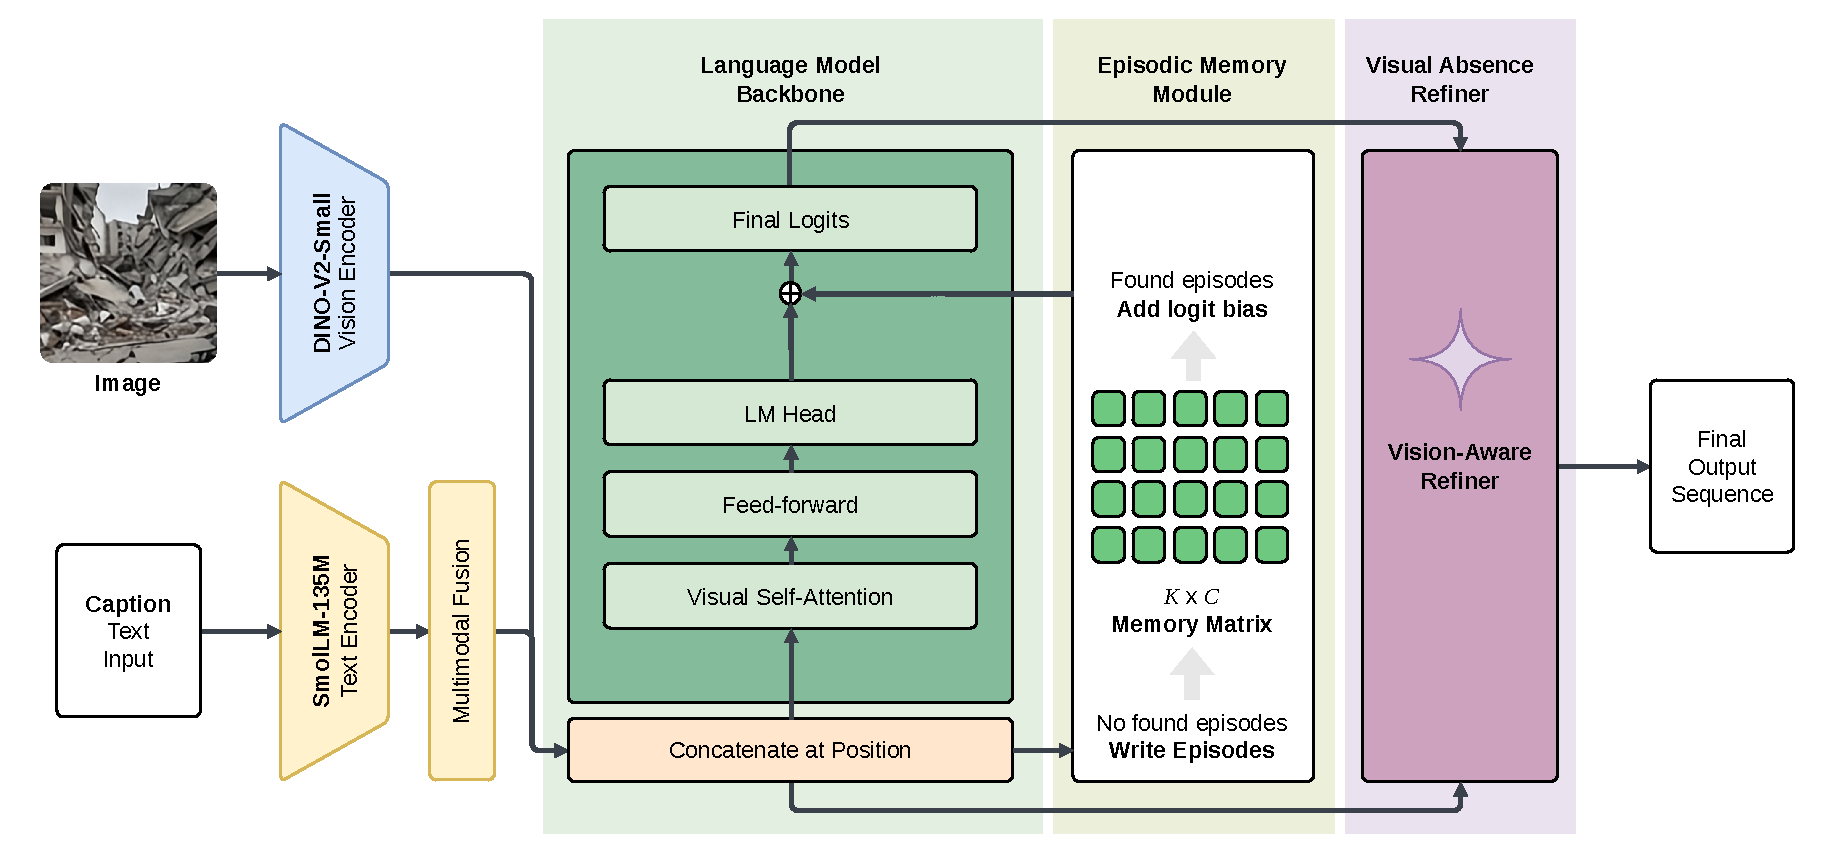
\includegraphics[width=\linewidth]{figures/main_diagram.pdf}
\end{minipage}
\caption{EmberVLM architecture overview. We introduce both episodic memory and the VA refiner module as part of the model.}
\label{fig:main}
\end{figure*}

Our core im is to maximize model capabilities under strict edge-deployment constraints. For our specific mission-critical evaluations, we adapt this base engine with a specialized task-specific routing head. The Episodic Memory and VA Refiner modules (detailed in Sec.~\ref{sec:memory} and \ref{sec:refiner}) seamlessly integrate into this backbone.

\paragraph{Base Multimodal Pipeline}
We employ DINO-V2-Small \cite{oquab2024dinov2learningrobustvisual} as our frozen visual perception module and SmolLM-135M \cite{allal2024SmolLM} as the text encoder. Unlike standard high-resolution VLM encoders, this backbone aggressively compresses an input image $X_v$ into a minimal sequence of $N_v = 8$ visual tokens ($d_{vis} = 384$). For the cognitive engine, we utilize TinyLLM-30M \cite{kandala2024tinyllmframeworktrainingdeploying}, a compact causal language model. To preserve linguistic priors while enabling multimodal adaptation under a strict parameter budget, the language backbone remains largely frozen and training only the final layer.

\paragraph{Stable Gated Fusion}
We project the raw visual tokens into the language dimension space ($d_{lang} = 384$) using a parameter-efficient bottleneck adapter ($d_{bottleneck} = 48$). We introduce an explicitly learnable vision gate scalar, $\alpha$ (initialized to $2.5$). The visual influence is dynamically scaled:
\begin{equation}
    V_{fused} = \sigma(\alpha) \cdot \text{LayerNorm}(V_{adapt})
\end{equation}
where $\sigma$ denotes the sigmoid activation. These gated visual tokens are subsequently interleaved with textual embeddings to form the joint context sequence processed by the language backbone.

\paragraph{Task-Specific Adaptation: Top-$K$ Robot Selection}
While EmberVLM is capable of standard autoregressive generation, generating raw text tokens is often inefficient and prone to formatting errors during mission-critical tactical deployment. For our primary autonomous robot selection task, we bypass the standard language modeling head. 

We aggregate the final hidden states from the language backbone via mean pooling into a dense, comprehensive incident representation, $h_{pool}$. We then attach a specialized \textit{Reasoning and Action Head}. This head processes $h_{pool}$ through a multi-layer perceptron (MLP) to output a probability distribution over the available robot fleet, naturally framing the deployment decision as a Top-$K$ classification task. This decoupling explicitly separates general scene comprehension from tactical execution, keeping the total trainable footprint strictly under 40M parameters while avoiding the latency of autoregressive decoding.

\subsection{Episodic Memory Module}
\label{sec:memory}

To enable dynamic adaptation and training-free knowledge updates at the edge, EmberVLM incorporates an Episodic Memory module. Let $z$ denote the final mean-pooled, fused multimodal embedding for a given incident. The memory system manages a fixed-size memory matrix $M \in \mathbb{R}^{K \times C}$, where $K=512$ denotes the number of experiential slots and $C=576$ represents the feature dimension, alongside an associated covariance matrix to track structural update statistics.

\paragraph{Scope Detection and Readout}
Before engaging retrieval, the incoming representation $z$ is evaluated by a lightweight \textit{Scope Detector}, implemented as a 2-layer MLP binary classifier. This detector outputs a probability $p(\text{in-scope})$ indicating whether the current incident falls within the domain of acquired memory. If $p < 0.5$, the query is deemed out-of-scope, and the model defaults strictly to parametric generation. 

If $p \geq 0.5$, the fast memory retrieval path activates. The controller computes normalized addressing weights $w_k$ over all $K$ slots using a Gaussian distance-based mechanism. The weight assigned to the $k$-th memory slot is computed as a scaled softmax over the squared $L_2$ distances between the query $z$ and each stored slot $M_j$:
\begin{equation}
    w_k = \frac{\exp\left(-\frac{\lVert z - M_k \rVert^2}{2\alpha \nu \tau}\right)}{\sum_{j=1}^K \exp\left(-\frac{\lVert z - M_j \rVert^2}{2\alpha \nu \tau}\right)}
\end{equation}
where $\alpha$, $\nu$, and $\tau$ represent the update strength, variance, and temperature scaling factors, respectively. The retrieved memory readout vector $z_m$ is aggregated via a weighted sum of the memory slots. This readout is passed through the language model's unembedding head and added residually to the raw predictive logits, organically biasing the final generation toward historically successful resolutions.

\paragraph{Novelty Detection and Dynamic Writes}
To safely accumulate new knowledge during deployment without catastrophic forgetting, the controller evaluates the novelty of each incoming embedding $z$, defined as $\sigma(z \mid M) = \min_k \lVert z - M_k \rVert^2$. If this novelty score exceeds a predefined threshold, the incident is classified as a fundamentally new experience. 

Instead of discarding this out-of-scope insight, the system executes a single-shot, recursive algebraic update. Using a linear solve over the residual difference between the new embedding and the current memory readout, it updates both $M$ and the covariance matrix. When the memory reaches its $K$-slot capacity, a hybrid Least Recently Used and Least Frequently Used (LRU-LFU) policy overwrites the least valuable slot.

\paragraph{Knowledge Consolidation}
During a periodic Stage 5 consolidation phase, the frozen memory matrix serves as a teacher. Using a Mean Squared Error (MSE) alignment loss, the explicitly retrieved knowledge is distilled directly into the model's parametric weights. This distillation process ensures that frequently accessed experiences become deeply ingrained in the base model, freeing up memory slots for new edge encounters.

\subsection{Visual Absence (VA) Refiner}
\label{sec:refiner}

To strictly enforce visual grounding in mission-critical deployments, EmberVLM incorporates a lightweight Visual Absence (VA) Refiner. Operating at inference time without requiring retraining, the VA refiner detect and suppress ungrounded tokens dynamically. It combines logit-space visual consistency, internal neuron-level activations, and temporal burst detection.

\paragraph{Dual-View Consistency and Internal Feature Extraction}
VA Refiner evaluates token grounding through two parallel pathways. The first pathway computes a logit-based visual consistency score. At each generation step, the model computes the predictive logits twice: once standardly with the visual context ($L_{vis}$), and once with the visual tokens ablated ($L_{ablated}$). The logit-based visual absence score, $s_{logit}$, is estimated by the discrepancy between these distributions:
\begin{equation}
    s_{logit} = 1.0 - \tanh(|L_{vis} - L_{ablated}|)
\end{equation}
A high $s_{logit}$ indicates that the token is equally likely to be generated with or without the image, suggesting weak visual grounding.

Simultaneously, the second pathway monitors the internal state of the language backbone. A feature extractor hooks into the Feed-Forward Network (FFN) modules across the middle decoder layers (layers 10 through 14), capturing the top-128 neuron activations per layer. These activations are processed by a lightweight Continuous MLP classifier to generate a neuron-based visual absence probability, $p_{neuron}$. 

The final visual absence probability for a given token, $p_{VA}$, is calculated as a convex combination of both signals:
\begin{equation}
    p_{VA} = \lambda \cdot p_{neuron} + (1 - \lambda) \cdot s_{logit}
\end{equation}
where $\lambda$ (defaulting to $0.5$) balances the internal representation confidence against output distribution consistency.

\paragraph{Type-Aware Intervention and Burst Detection}
 EmberVLM applies token-type-aware thresholding. Using a heuristic dictionary of visually sensitive keywords (e.g., objects, colors, spatial relations), sensitive tokens are subjected to a strict hallucination threshold ($p_{VA} \geq 0.6$), whereas non-visual tokens are granted a looser boundary ($p_{VA} \geq 0.8$). Tokens exceeding their respective thresholds receive a severe logit penalty, forcing the model to select a more visually grounded alternative.

Since hallucinations often occur in cascading clusters, the VA Refiner maintains a sliding-window temporal memory of recent $p_{VA}$ scores. If the moving average exceeds a predefined burst threshold, the refiner escalates its intervention from a soft penalty to a hard block (setting the offending token's logit to $-\infty$) and dampens the broader output distribution to break the generative momentum of the hallucination cycle.

\paragraph{Mission Uncertainty Calibration}
After a full sequence is formulated, the system aggregates the $p_{VA}$ scores for all visually sensitive tokens. If the average absence score falls within a critical boundary, the refiner triggers a system-level uncertainty flag. Rather than prepending conversational caveats to the text, this flag signals the downstream autonomous controller that the current visual-tactical alignment is low-confidence, allowing the system to request a secondary camera angle or defer to human operator judgment.

\subsection{Training Curriculum}
\label{sec:training}

We use the AdamW optimizer with a learning rate of $2 \times 10^{-4}$ and an effective batch size of 256 for the foundational stages, which is subsequently halved during the complex reasoning stages to accommodate escalating memory requirements. Training runs are conducted in BFloat16 (bf16) mixed precision. The training datasets and epoch distributions are detailed in Table~\ref{tab:all_training_datasets}.

\begin{table}[ht]
\centering
\caption{EmberVLM Training Datasets Across All Stages}
\label{tab:all_training_datasets}
\begin{tabular}{llc}
\toprule
\textbf{Stage} & \textbf{Dataset Name} & \textbf{Epochs} \\
\midrule
\multirow{8}{*}{1: Alignment} 
& CC3M \cite{sharma-etal-2018-conceptual} & 10 \\
& RefCOCO \cite{yu2016modelingcontextreferringexpressions} & 10 \\
& VQA v2 \cite{VQA} & 10 \\
& COCO Annotations \cite{lin2015microsoftcococommonobjects} & 10 \\
& LLaVA \cite{liu2023visualinstructiontuning} & 10 \\
& OK-VQA \cite{marino2019okvqavisualquestionanswering} & 10 \\
& A-OKVQA \cite{schwenk2022aokvqabenchmarkvisualquestion} & 10 \\
& GQA \cite{hudson2019gqanewdatasetrealworld} & 10 \\
\midrule
2: Instruction Tuning & LLaVA Instruct 150K & 15 \\
\midrule
3: Task Adaptation & Robot Selection & 20 \\
\midrule
4: Latent CoT & Robot Selection (CoT) & 10 \\
\bottomrule
\end{tabular}
\end{table}

\subsubsection{Stage 1: Visual-Language Alignment}
We keep the vision and language backbones remain frozen. only the Fusion Module is actively trained. The model learns to map raw visual features into meaningful linguistic tokens by predicting captions and answering standard visual queries.

\subsubsection{Stage 2: Multimodal Instruction Tuning}
The second stage shifts the objective from foundational alignment to complex instruction following and visual dialogue. The vision encoder remains frozen, but both the Fusion Module and the Language Backbone are fully unfrozen and fine-tuned end-to-end. This enables the model to interpret nuanced human instructions and engage in multi-turn conversations grounded in visual context.

\subsubsection{Stage 3: Robot Fleet Selection}
The model is trained to analyze incident scenes and select the most appropriate robotic asset from a predefined fleet (e.g., Drone, Underwater Robot, Humanoid, Wheeled, Legged). The standard autoregressive head is bypassed, and the \textit{Reasoning and Action Head} is unfrozen and trained alongside the core model using cross-entropy loss. Due to the specialized nature of the task.

\subsubsection{Stage 4: Latent Chain-of-Thought Integration}
The final supervised stage instills deductive transparency without incurring the severe latency penalties of autoregressive text generation. Rather than predicting explicit text tokens, the \textit{Reasoning Head} is trained to align its internal step-embeddings with procedurally generated Chain-of-Thought (CoT) rationales using a contrastive loss.

\section{Experiments}
\label{sec:experiments}
\subsection{Baseline Comparisons and Generalization}
\label{sec:baselines}

Performance of EmberVLM on multimodal datasets are presented in Table~\ref{tab:episodic_memory_gen_tasks}. While larger models naturally possess greater raw capacity and score higher on generic benchmarks, their massive memory footprints and latency make them categorically unsuited for the edge environments targeted by EmberVLM.

Beyond the mission-critical robotics benchmarks, it is essential to verify that our aggressive architectural compression and targeted memory modules do not degrade general vision-language capabilities. Table~\ref{tab:episodic_memory_gen_tasks} also shows the impact of the episodic memory module across standard multimodal reasoning and coherence metrics.

\begin{table}[ht]
\centering
\caption{EmberVLM evaluation on diverse multimodal tasks.}
\label{tab:episodic_memory_gen_tasks}
\begin{tabular}{lcc}
\toprule
\textbf{Metric} & \textbf{No Memory} & \textbf{With Memory} \\
\midrule
Coherence aggregate score & 13.1 & \textbf{17.1} \\
GQA VQA \cite{hudson2019gqanewdatasetrealworld} & 10.0\% & 10.0\% \\
UniBench \cite{altahan2024unibenchvisualreasoningrequires} & 7.0\% & \textbf{8.0\%} \\
SugarCrepe \cite{hsieh2023sugarcrepefixinghackablebenchmarks}& 14.0\% & \textbf{16.0\%} \\
\midrule
Extra FLOPs per step & \textbf{0} & $\sim$0.3-0.6M \\
Episodic memory RAM & \textbf{0} & $\sim$1.2 MB \\
\bottomrule
\end{tabular}
\end{table}

The integration of the episodic memory yields consistent improvements across the board. Most notably, the Coherence Aggregate Score improves by over 30\% (from 13.1 to 17.1). The model also demonstrates stable gains on broader multimodal benchmarks, including a 14.2\% relative improvement on SugarCrepe (14.0\% to 16.0\%) and a 1-point absolute gain on UniBench, while maintaining strict parity on GQA.

Crucially, these gains are achieved with virtually zero computational penalty. As detailed in the lower section of Table~\ref{tab:episodic_memory_gen_tasks}, the episodic memory module introduces only $\sim$1.2 MB of static RAM overhead and approximately 0.3 to 0.6M extra FLOPs per inference step. This results in a vastly superior quality-to-compute ratio (17.1/1.03 vs. 13.1/1.0), proving that EmberVLM's dynamic memory caching is a highly optimal strategy for scaling reasoning capabilities without violating edge-deployment constraints.

\subsection{Edge Deployment and Dynamic Memory Management}
\label{sec:edge_deployment}

In mission-critical edge scenarios, managing the active memory footprint (e.g., VRAM or SRAM) is often just as critical as minimizing computational latency. To accommodate severely resource-constrained hardware, EmberVLM employs a dynamic, tiered memory management strategy during deployment. 

Rather than pinning the entire 164M-parameter architecture in active compute memory, the system leverages the episodic memory module as a high-speed experiential cache. The lightweight scope detector and the $512 \times 576$ memory matrix are permanently pinned to the primary compute device. For historically seen instances—where the scope detector registers a high confidence—the system directly retrieves the necessary contextual biases and execution plans. 

Concurrently, the model's parametric weights are maintained in secondary storage. By dynamically loading only the necessary active components, EmberVLM achieves an significant reduction in the active memory footprint. This architecture effectively frees up critical on-device memory, allowing the main inference operations to run smoothly.

\begin{table}[t]
\centering
\caption{Training carbon emissions from CodeCarbon integration. All values are \textbf{measured}, not estimated. Training was conducted on a dual-GPU distributed setup (2 ranks). Stages 3--4 contribute negligible emissions relative to alignment and instruction tuning.}
\label{tab:emissions}
\begin{tabular}{lrrr}
\toprule
\textbf{Stage} & \textbf{Duration (est.)} & \textbf{Emissions (kg CO$_2$eq)} & \textbf{\% of Total} \\
\midrule
Stage 1 --- Alignment       & 50 h (5 epochs)   & 16.6513 & 65.6\% \\
Stage 2 --- Instruction     & 40 h (13 epochs)  & 8.6545  & 34.1\% \\
Stage 3 --- Robot Selection & $\approx$20 min   & 0.0046  & 0.02\% \\
Stage 4 --- Reasoning       & $\approx$10 min   & 0.0062  & 0.02\% \\
\midrule
\textbf{Total}             & \textbf{$\approx$90 h} & \textbf{25.3166} & \textbf{100\%} \\
\bottomrule
\end{tabular}
\end{table}
\subsection{Mission Critical Evaluation}

Table~\ref{tab:robot_selection} presents the primary ablation results on the 103-sample robot-selection validation split.

\begin{table}[t]
\centering
\caption{Robot fleet selection ablation on the 103-sample validation split. Episodic memory adds a single $512 \times 576$ read operation per query. Abs. $\Delta$ represents the absolute metric improvement. ECE: lower is better ($\downarrow$); all others: higher is better ($\uparrow$).}
\label{tab:robot_selection}
\begin{tabular}{lccc}
\toprule
\textbf{Metric} & \textbf{NoMemory} & \textbf{YesMemory} & \textbf{Abs. $\Delta$} \\
\midrule
Validation accuracy & 0.0971 & 0.5437 & $+0.4466$ \\
Macro precision & 0.0194 & 0.2811 & $+0.2617$ \\
Macro recall & 0.2000 & 0.3458 & $+0.1458$ \\
Macro F1 & 0.0354 & 0.2970 & $+0.2616$ \\
Expected calibration error (ECE) $\downarrow$ & 0.3409 & 0.1849 & $-0.1560$ \\
Multi-robot exact match & 0.0097 & 0.0874 & $+0.0777$ \\
Multi-robot Jaccard & 0.0097 & 0.2961 & $+0.2864$ \\
\bottomrule
\end{tabular}
\end{table}

Without experiential conditioning, the baseline (NoMemory) suffers from severe model collapse, degrading into a near single-class predictor. It heavily over-indexes on the "Robot-with-Wheels" class (Recall = 1.0, F1 = 0.1770), while entirely failing on all other classes (Drone, Underwater Robot, Humanoid, Robot-with-Legs yield F1 = 0.0). 

Conversely, the episodic variant successfully breaks this collapse and discriminates across multiple morphologies. It achieves strong performance on the Drone class (F1 = 0.6667; Precision = 0.5054, Recall = 0.9792) and the Underwater Robot class (F1 = 0.8182; Precision = 0.9000, Recall = 0.7500). We note that the Humanoid and Robot-with-Legs classes remain at F1 = 0.0 for both variants. However, rather than indicating a failure of the memory conditioning, this directly reflects the extreme scarcity of these specific asset classes within the 103-sample validation split.

\paragraph{Out-of-Domain Generalization}
To validate EmberVLM's robustness beyond the primary top-$N$ robot-selection setting, we benchmark the model on two additional mission-critical datasets: VERI-Emergency for visual emergency recognition~\cite{choi2026better} and GEO-Bench-VLM for geospatial disaster understanding~\cite{danish2025geobench}. These tasks assess whether our edge-oriented design transfers to safety-relevant domains beyond robot assignment.

As shown in Table~\ref{tab:risk_benchmark_results}, EmberVLM demonstrates highly competitive out-of-domain generalization despite being the most compact model evaluated. Notably, EmberVLM achieves the highest accuracy on both VERI-Emergency (0.6400) and GEO-Bench-VLM (0.7200). We also observe that iterative suppression of low-confidence tokens improves reliability, with a modest latency trade-off.

\begin{table*}[t]
    \centering
    \caption{Performance comparisons on mission-critical visual recognition benchmarks.}
    \label{tab:risk_benchmark_results}
    \resizebox{\textwidth}{!}{
    \begin{tabular}{l|ccc|ccc|cc}
        \toprule
        \multirow{2}{*}{\textbf{Model}} & \multicolumn{3}{c|}{\textbf{Top-$N$ Robot Selection}} & \multicolumn{3}{c|}{\textbf{VERI-Emergency}} & \multicolumn{2}{c}{\textbf{GEO-Bench-VLM}} \\
        \cmidrule(lr){2-9}
        & ExactAcc. & Macro-F1 & Time(s) & Acc. & OverRx & UnderRx & Acc. & Time(s) \\
        \midrule
        InternVL3-1B & 0.0720 & 0.1748 & \textbf{187.5} & 0.6350 & 0.6600 & \textbf{0.0700} & 0.3772 & 1051.7 \\
        MobileVLM\_V2-1.7B & 0.0960 & 0.2294 & 271.6 & 0.5350 & 0.4700 & 0.4600 & 0.1896 & \textbf{175.0} \\
        SmolVLM-256M & 0.0000 & 0.1391 & 557.4 & 0.4950 & 0.0100 & 1.0000 & 0.2066 & 2001.4 \\
        SmolVLM2-256M & 0.0000 & 0.2254 & 513.9 & 0.5000 & \textbf{0.0000} & 1.0000 & 0.2383 & 1834.7 \\
        \midrule
        \textbf{EmberVLM NoMem} & 0.0960 & 0.2350 & 3641.8 & 0.4700 & 0.7700 & 0.2900 & 0.2086 & 6244.3 \\
        \textbf{EmberVLM} & \textbf{0.2100} & \textbf{0.4200} & 2381.9 & \textbf{0.6400} & 0.5200 & 0.1400 & \textbf{0.7200} & 2247.7 \\
        \bottomrule
    \end{tabular}
    }
\end{table*}


\subsection{Episodic Memory Module}
Table~\ref{tab:robot_selection} and Table~\ref{tab:risk_benchmark_results} summarises the episodic memory
ablation across all evaluated dimensions. The two configurations
are trained with identical hyperparameters, identical teacher model
(Qwen2-VL-7B for Stage-2 distillation), and evaluated on identical
held-out splits. We can see that the model with episodic memory actually gains performance and being faster than the part which doesn't include episodic memory.

\subsection{Hallucination Mitigation and Mechanistic Analysis}
\label{sec:eval_hallucination}

To evaluate the efficacy of the Visual Absence (VA) Refiner, we assess EmberVLM's generation both with and without the plug-and-play module active at inference time. Across our core mission-critical evaluation split, the application of the VA Refiner achieves a significant reduction in ungrounded token generation without modifying any underlying model weights or incurring retraining costs. 

To validate these gains on standardized benchmarks, we further evaluated the model on a 100-sample subset of the POPE Adversarial dataset, a rigorous benchmark designed specifically to probe object hallucination. The presence of the VA Refiner drops the absolute hallucination rate from 29\% to 24\%, while concurrently boosting overall accuracy from 64\% to 68\%, proving that suppressing ungrounded tokens directly correlates with improved downstream task performance.

\paragraph{Mechanistic Interpretability of Hallucinations}
Beyond quantitative metrics, we visually analyze the internal dynamics that drive the VA Refiner's efficacy. Figure~\ref{fig:neuron} illustrates the activation patterns of the SmolLM-135M mid-decoder MLP neurons under two conditions: standard multimodal inference and visually-ablated inference.

\begin{figure*}[t]
\centering
\begin{minipage}{\textwidth}
\centering
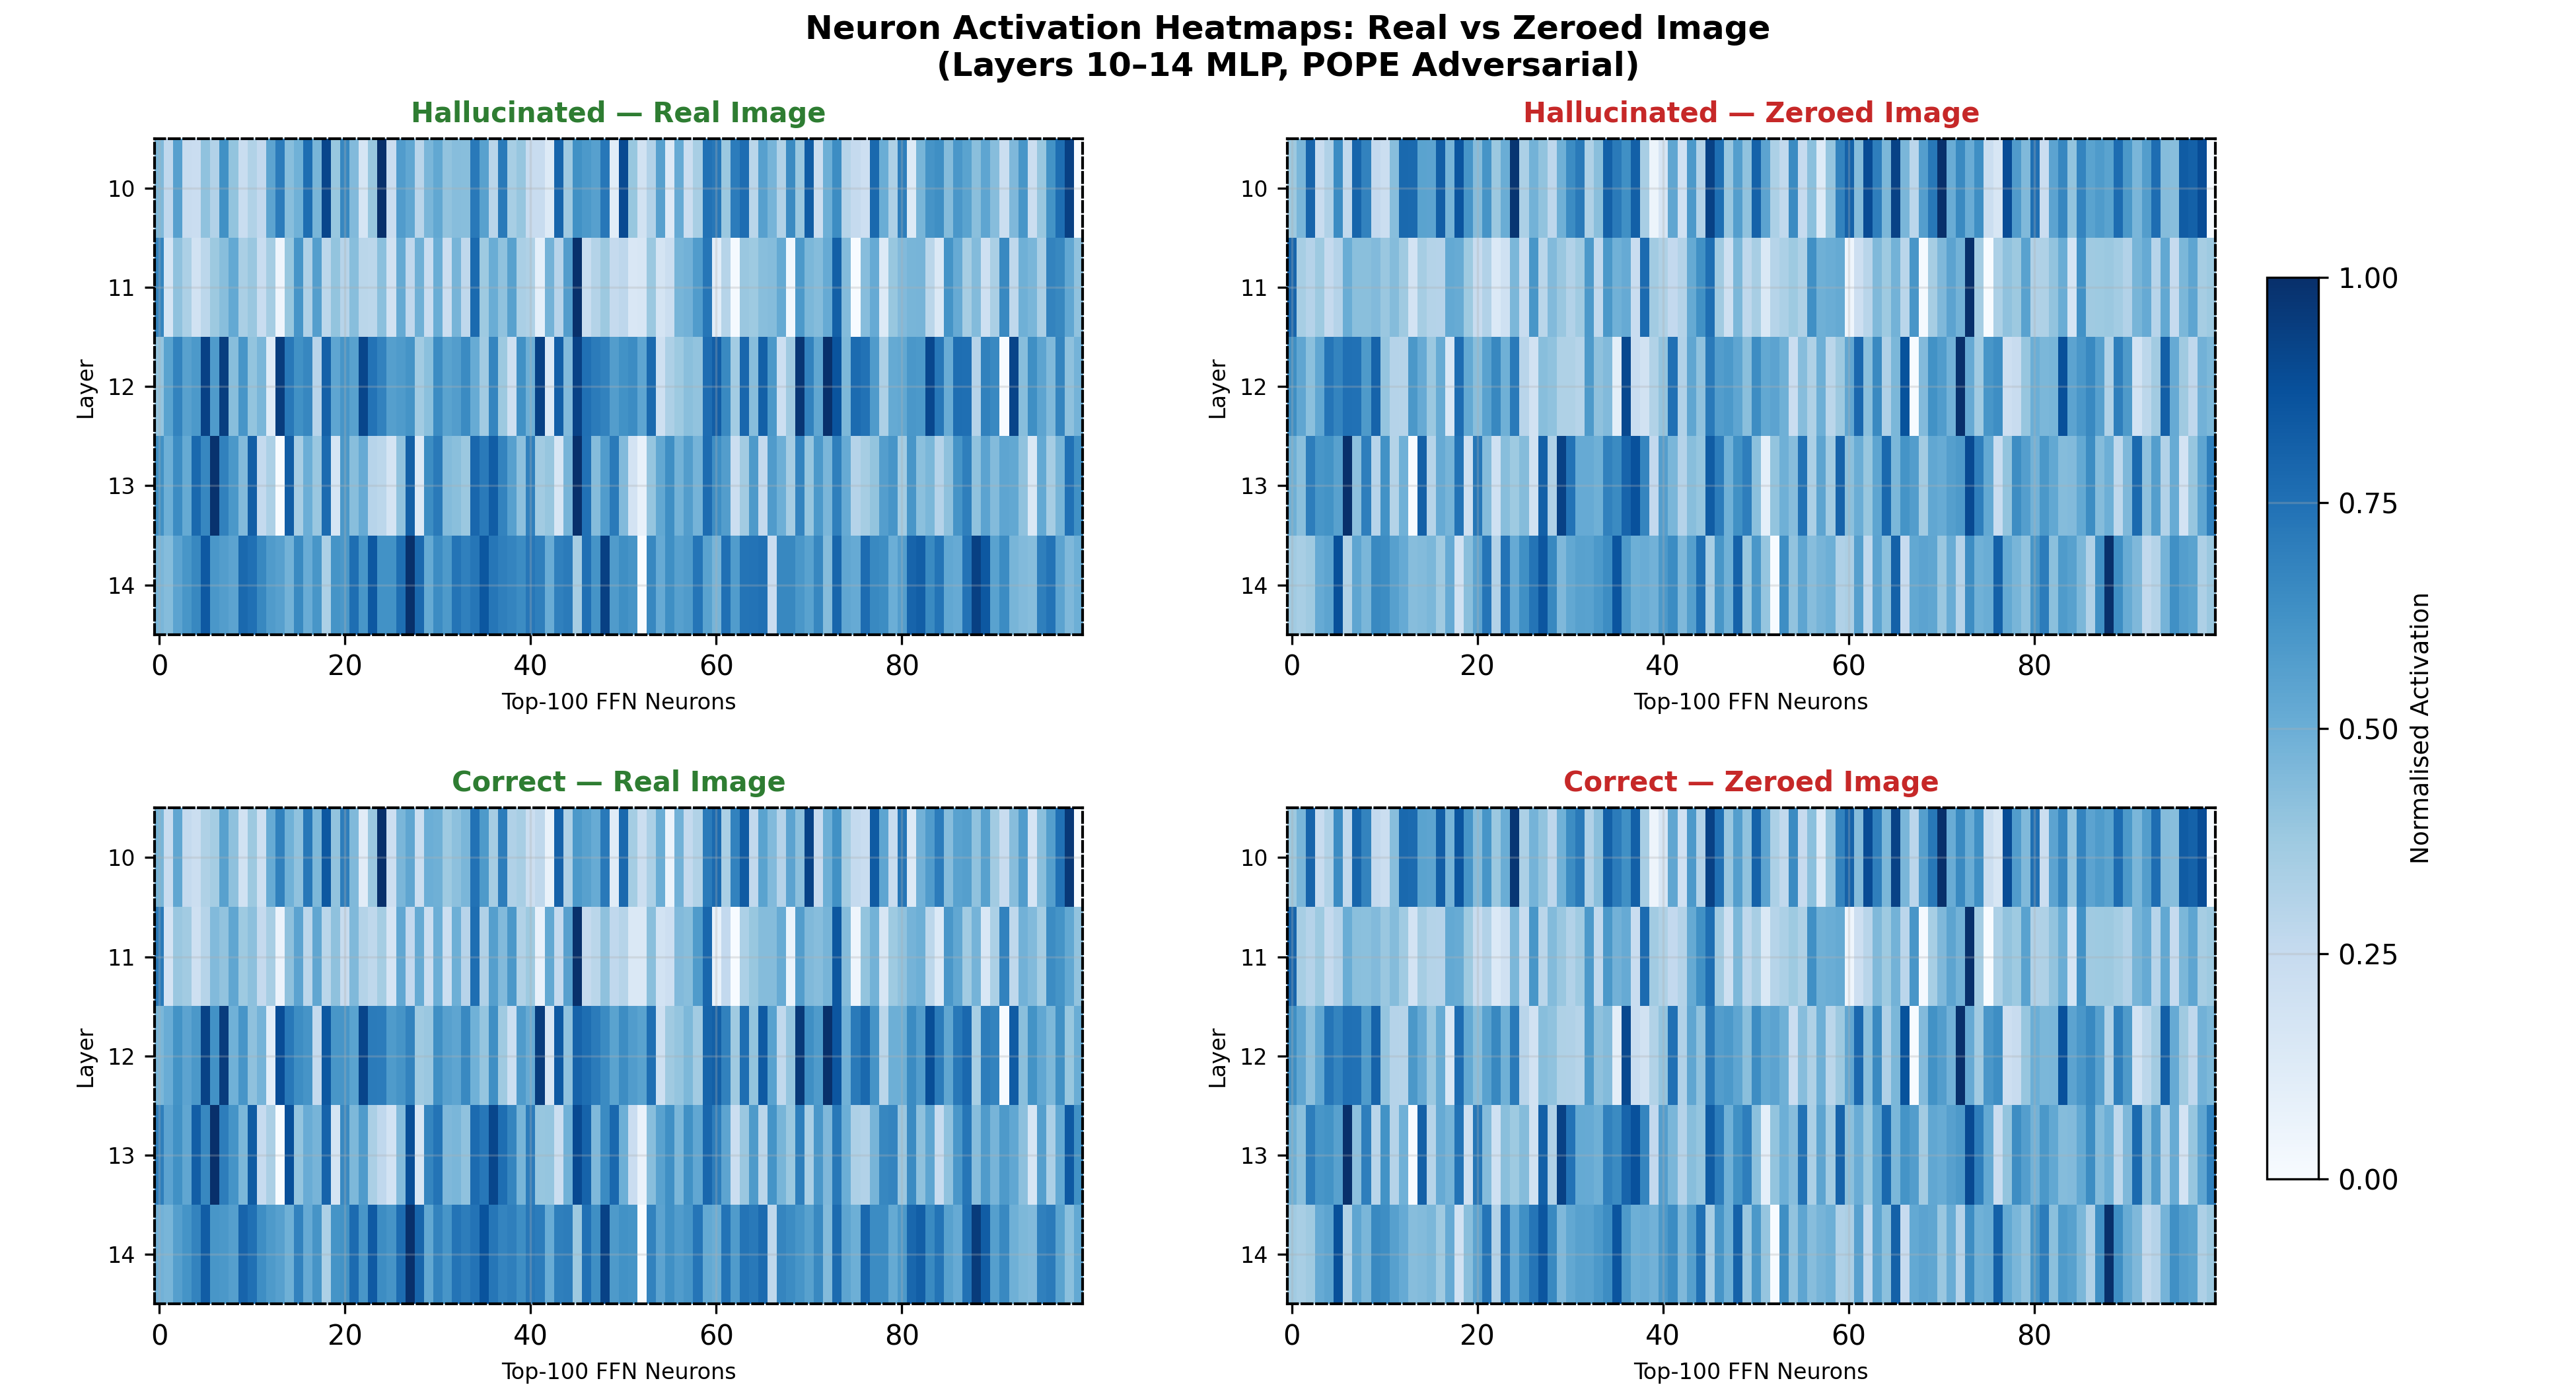
\includegraphics[width=\linewidth]{figures/va_ablation_neuron_heatmap.png}
\end{minipage}
\caption{Neuron activation heatmaps comparing visually grounded and hallucinated tokens. \textbf{Top:} For hallucinated cases, activation patterns remain nearly identical regardless of the visual input's presence, indicating the model is generating text based entirely on language priors. \textbf{Bottom:} For correctly grounded cases, activation patterns heavily diverge when the image is removed, demonstrating a strong structural reliance on actual visual content.}
\label{fig:neuron}
\end{figure*}

This visualization reveals the precise internal mechanism behind object hallucination. For hallucinated generations (Fig.~\ref{fig:neuron}, top row), the neuron activation patterns remain highly symmetric regardless of whether the visual input is present. This indicates that these specific neurons fire independently of the visual context, relying entirely on the language model's pretrained semantic priors to "guess" an appropriate token. 

Conversely, for correct, visually grounded generations (Fig.~\ref{fig:neuron}, bottom row), the activation patterns change drastically when the image is removed. This noticeable divergence confirms that these neurons depend structurally on the actual image content to formulate an answer. By dynamically monitoring these exact discrepancies across layers 10 through 14, the VA Refiner successfully isolates and penalizes tokens driven by language priors rather than visual evidence.

\subsection{Carbon Footprint}
\label{sec:emissions}

The scaling of Vision-Language Models has brought substantial energy consumption
and carbon emissions, making compute efficiency an increasing priority, particularly
for edge-oriented models where efficiency is a core requirement.

EmberVLM's compact, parameter-efficient design drastically reduces both energy use
and carbon footprint compared to billion-parameter baselines. As shown in
Table~\ref{tab:emissions}, training completes on a standard dual-GPU node,
accelerating iteration while keeping the lifecycle of edge AI environmentally
sustainable.

\subsection{Experiment Setup}

All the training was conducted in 2xA100 GPUs, while inferences is done in AMD Ryzen 3 4100 4-Core Processor 3.80 GHz CPU with 32GB of RAM. 


\section{Discussion and Limitations}
\label{sec:discussion}

EmberVLM demonstrates that reliable, low-latency multimodal reasoning on resource-constrained edge devices does not strictly require massive parameter scaling. By utilizing a tiered Episodic Memory module, the architecture actively breaks the traditional latency-accuracy tradeoff. It successfully prevents the single-class collapse observed in memory-free baselines and achieves competitive out-of-domain generalization on emergency benchmarks, all while reducing evaluation latency and maintaining a  smaller active memory footprint (with only 1.2~MB static overhead). Furthermore, the Visual Absence Refiner provides a mechanistically grounded safeguard against catastrophic hallucinations. By penalizing mid-decoder neurons that over-rely on semantic priors rather than visual evidence, it penalizes ungrounded tokens and significantly improves adversarial robustness. Crucially, these capabilities are achieved with a remarkably low environmental footprint; strictly limiting trainable parameters to under 40M yields total measured training emissions of just 25.3~kg CO$_2$eq, providing a highly sustainable blueprint for Green AI.

Despite these strengths, inherent limitations remain. The fixed capacity of the episodic memory matrix ($K=512$ slots) relies heavily on the LRU-LFU replacement policy and may eventually saturate in highly diverse, open-world deployments. Future work should explore dynamically expandable or hierarchical memory structures. Additionally, relying on a highly compressed, frozen visual encoder (DINOv2-Small) inherently precludes the dense, high-resolution spatial granularity required for microscopic or extreme long-range visual inspection tasks. Expanding the VA Refiner's temporal burst detection into a fully multi-agent verification loop also presents a promising avenue for zero-tolerance safety applications.

\section{Limitations}

Three limitations require acknowledgment. First, the episodic
memory buffer (512 slots, 576-dim, $\approx$1.2~MB fp32) is
fixed in size at deployment. If the operating environment changes
substantially over time, stale episodes may degrade retrieval
quality. The LRU+LFU replacement policy mitigates this, but
adaptive memory management under non-stationary distributions
remains an open problem. Second, the Visual Absence Refiner hooks
into decoder MLP layers 10--14 of SmolLM-135M and relies on
neuron-level activation patterns specific to this architecture.
Reapplying the refiner to a different LM backbone requires
re-identifying the relevant hook layers and re-calibrating the
visual-absence classifier.

\section{Future Work}

Future directions include: (i) adaptive episodic memory management
that dynamically resizes the buffer based on device memory
availability and environmental novelty signals; (ii) cross-backbone
transfer of the Visual Absence Refiner via activation alignment
rather than layer-specific hooks; and (iii) extending the
robot-selection evaluation to larger and more diverse mission
datasets to assess generalisation beyond the 103-sample validation
split used in this work.

\section{Conclusion}
\label{sec:conclusion}

In this work, we presented EmberVLM, a highly compact and parameter-efficient vision-language architecture purpose-built for mission-critical edge deployments. By deliberately stepping away from the paradigm of massive parameter scaling, we demonstrated that advanced, reliable multimodal reasoning can be achieved under severe hardware constraints. The integration of our dynamic Episodic Memory module effectively breaks the traditional latency-accuracy trade-off, enabling training-free experiential caching that significantly boosts downstream performance on complex tasks—such as autonomous robot selection—while reducing the active memory footprint. 

Furthermore, the introduction of the training-free Visual Absence (VA) Refiner provides a robust, mechanistically grounded safeguard against catastrophic hallucinations, suppressing visually ungrounded tokens significantly. Validated across diverse emergency and disaster recognition benchmarks, EmberVLM not only achieves state-of-the-art reliability for sub-billion parameter models but accomplishes this with a rigorously measured, remarkably low carbon footprint. Ultimately, EmberVLM offers a sustainable, high-performance blueprint for the future of safe and deployable AI at the edge.

% ---- Bibliography ----
%\bibliographystyle{splncs04}
%\bibliography{main}
% ---- Bibliography ----
%
% BibTeX users should specify bibliography style 'splncs04'.
% References will then be sorted and formatted in the correct style.
%
\bibliographystyle{splncs04}
\bibliography{main}
\end{document}
